% Format teze zasnovan je na paketu memoir
% http://tug.ctan.org/macros/latex/contrib/memoir/memman.pdf ili
% http://texdoc.net/texmf-dist/doc/latex/memoir/memman.pdf
% 
% Prilikom zadavanja klase memoir, navedenim opcijama se podešava 
% veličina slova (12pt) i jednostrano štampanje (oneside).
% Ove parametre možete menjati samo ako pravite nezvanične verzije
% mastera za privatnu upotrebu (na primer, u b5 varijanti ima smisla 
% smanjiti 
\documentclass[12pt,oneside]{memoir} 

% Paket koji definiše sve specifičnosti master rada Matematičkog fakulteta
\usepackage[latinica,biblatex]{matfmaster} 
%
% Podrazumevano pismo je ćirilica.
%   Ako koristite pdflatex, a ne xetex, sav latinički tekst na srpskom jeziku
%   treba biti okružen sa \lat{...} ili \begin{latinica}...\end{latinica}.
%
% Opicija [latinica]:
%   ako želite da pišete latiniciom, dodajte opciju "latinica" tj.
%   prethodni paket uključite pomoću: \usepackage[latinica]{matfmaster}.
%   Ako koristite pdflatex, a ne xetex, sav ćirilički tekst treba biti
%   okružen sa \cir{...} ili \begin{cirilica}...\end{cirilica}.
%
% Opcija [biblatex]:
%   ako želite da koristite reference na više jezika i umesto paketa
%   bibtex da koristite BibLaTeX/Biber, dodajte opciju "biblatex" tj.
%   prethodni paket uključite pomoću: \usepackage[biblatex]{matfmaster}
%
% Opcija [b5paper]:
%   ako želite da napravite verziju teze u manjem (b5) formatu, navedite
%   opciju "b5paper", tj. prethodni paket uključite pomoću: 
%   \usepackage[b5paper]{matfmaster}. Tada ima smisla razmisliti o promeni
%   veličine slova (izmenom opcije 12pt na 11pt u \documentclass{memoir}).
%
% Naravno, opcije je moguće kombinovati.
% Npr. \usepackage[b5paper,biblatex]{matfmaster}

% Pomoćni paket koji generiše nasumičan tekst u kojem se javljaju sva slova
% azbuke (nema potrebe koristiti ovo u pravim disertacijama)
\usepackage[latinica]{pangrami}

% Datoteka sa literaturom u BibTex tj. BibLaTeX/Biber formatu
\bib{matfmaster-primer}

% Ime kandidata na srpskom jeziku (u odabranom pismu)
\autor{Đorđe Todorović}
% Naslov teze na srpskom jeziku (u odabranom pismu)
\naslov{Poboljšanje GNU GDB alata prilikom analize TLS promenljivih pomoću datoteka jezgara generisanih na ugrađenim uređajima drugih arhitektura}
% Godina u kojoj je teza predana komisiji
\godina{2018}
% Ime i afilijacija mentora (u odabranom pismu)
\mentor{dr Mika \textsc{Mikić}, redovan profesor\\ Univerzitet u Beogradu, Matematički fakultet}
% Ime i afilijacija prvog člana komisije (u odabranom pismu)
\komisijaA{dr Ana \textsc{Anić}, vanredni profesor\\ University of Disneyland, Nedođija}
% Ime i afilijacija drugog člana komisije (u odabranom pismu)
\komisijaB{dr Laza \textsc{Lazić}, docent\\ Univerzitet u Beogradu, Matematički fakultet}
% Ime i afilijacija trećeg člana komisije (opciono)
% \komisijaC{}
% Ime i afilijacija četvrtog člana komisije (opciono)
% \komisijaD{}
% Datum odbrane (odkomentarisati narednu liniju i upisati datum odbrane ako je poznat)
% \datumodbrane{}

% Apstrakt na srpskom jeziku (u odabranom pismu)
\apstr{%
\pangrami
}

% Ključne reči na srpskom jeziku (u odabranom pismu)
\kljucnereci{analiza, geometrija, algebra, logika, računarstvo, astronomija}

\begin{document}
% ==============================================================================
% Uvodni deo teze
\frontmatter
% ==============================================================================
% Naslovna strana
\naslovna
% Strana sa podacima o mentoru i članovima komisije
\komisija
% Strana sa posvetom (u odabranom pismu)
\posveta{Mami, tati i dedi}
% Strana sa podacima o disertaciji na srpskom jeziku
\apstrakt
% Sadržaj teze
\tableofcontents*

% ==============================================================================
% Glavni deo teze
\mainmatter
% ==============================================================================

% ------------------------------------------------------------------------------
\chapter{Uvod}
% ------------------------------------------------------------------------------

% ------------------------------------------------------------------------------

\chapter{Kako rade debageri?}
\label{chp:debageri}

Debager (eng. \emph{debagger}) je softverski alat koji koriste programeri za testiranje, analizu i otklanjanje grešaka u programima. Sam proces korišćenja takvih alata nazivamo debagovanjem (eng. \emph{debugging}).
Debageri mogu startovati neki proces i debagovati ga, ili "nakačiti" se na neki proces koji je već u fazi rada. Kada isti preuzme kontrolu nad programom može ga izvršavati instrukciju po instrukciju, postavljati tačke prekida (eng. \emph{brakpoints}) itd. Neki debageri imaju mogućnost da izvrše neke posebne izraze ili funkcije adresnog prostora programa koji se debaguje, ili čak menjati strukturu programa prateći propratne efekte.

Podršku debagerima, u opštem slučaju, svakako daju operativni sistemi, kroz sistemske pozive koji omogućavaju tim alatima da pokrenu i preuzmu kontrolu nad nekim drugim procesom.

\section{Linux Debageri}

Pre svega, definišimo neke od osnovnih pojmova Linux programiranja koje ćemo često pominjati u radu.
Osvrnimo se prvo na ELF (eng. \emph{Executable and Linkable Format}) fajl format izvršnih fajlova, deljenih biblioteka, objektnih fajlova i datoteka jezgara. ELF sadrži razne informacije o samom fajlu koji je podeljen u dva dela: ELF zaglavlje i podaci fajla. ELF zaglavlje sadrži informacije o arhitekturi za koju je program preveden i definiše da li program koristi 32-bitni ili 64-bitni adresni prostor. Zaglavlje 32-bitnih programa je dužine 52 bajta, dok kod 64-bitnih programa isti je dužine 64 bajta. Podaci fajla mogu sadržati programsku tabelu zaglavlja (eng. \emph{Program header table}), sekcijisku tabelu zaglavlja (eng. \emph{Section header table}) i ulazne tačke prethodne dve tabele.

\begin{figure}[h!]
	\begin{center}
		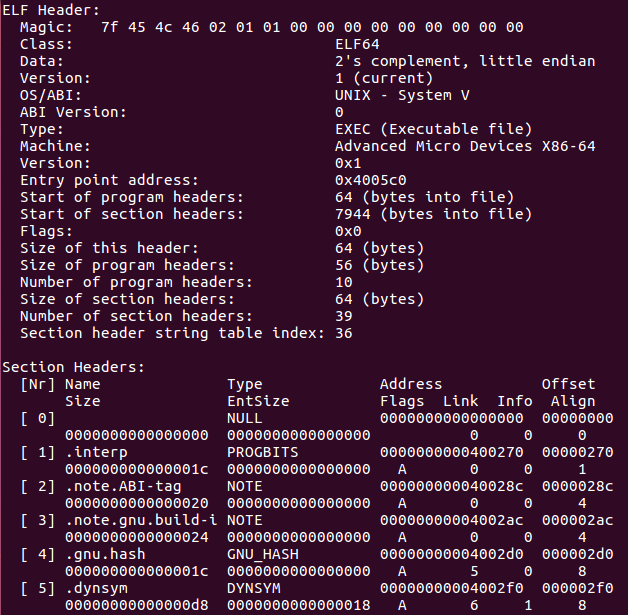
\includegraphics[scale=0.5]{slike/elf_example.png}
	\end{center}
	\caption{ELF fajl format}
	\label{fig:elf}
\end{figure}

Nakon ELF fajl formata, jako bitan fajl format je DWARF, koji predstavalja format zapisa debag informacija koje debageri koriste kada analiziraju programe. DWARF je od posebne važnosti za rad te će isti biti opisan detaljnije u nastavku.

GNU Linux operativni sistem pruža sistemski poziv \emph{ptrace} koji zapravo debagerima omogućava rad. Ovaj sistemski poziv omogućava jednom procesu kontrolu nad izvršavanjem nekog drugog procesa i menjanje memroije i registara istog.
\newline\newline
\emph{ long ptrace(enum \_\_ptrace\_request request, pid\_t pid, void *addr, void *data);}
\newline

Prvi argument sistemskog poziva predstavlja zapravo informaciju kojom operativnom sistemu jedan proces, ne nužno debager, ukazuje na nameru preuzimanja kontrole drugog procesa. Neki od njih su:

\begin{enumerate}
	\item PTRACE\_TRACEME - omogućava praćenje (eng. \emph{tracing})
	\item PTRACE\_PEEKDATA - čitanje memorije
	\item PTRACE\_POKEDATA - pisanje memorije
	\item PTRACE\_GETREGS - čitanje registara
	\item PTRACE\_SETREGS - pisanje registara
\end{enumerate}
Drugi argmunet sistemskog poziva \emph{pid} ukazuje na identifikacioni broj ciljanog procesa, dok treći i četvrti argument se po potrebi koriste u zavisnosti od namere korišćenja \emph{ptrace} sistemskog poziva. 
\subsection{Tačke prekida}

Postoje dve vrste tačaka prekida (eng. \emph{brakpoints}): softverske i hardverske.

Osvrnimo se prvo na softverske tačke prekida. Postavljanje tačaka prekida predstavlja jednu od najkorišćenijih mogućnosti debagera, te stoga navedimo par smernica kako je ista realizovana, u opštem slučaju. Ali takođe treba napomenuti da ne postoji jedinstveni poziv nekog sistemskog poziva za postavljanje tačke prekida, već se ista obavlja kao kombinacija više mogućnosti \emph{ptrace} sistemskog poziva. Opišimo ceo postupak na jednostavnom primeru. Program je preveden za Intel x86-64 procesorsku arhitekturu i asemblerski kod \emph{main} funkcije primera izgelda kao na slici \ref{fig:primer1}.

\begin{figure}[h!]
	\begin{center}
		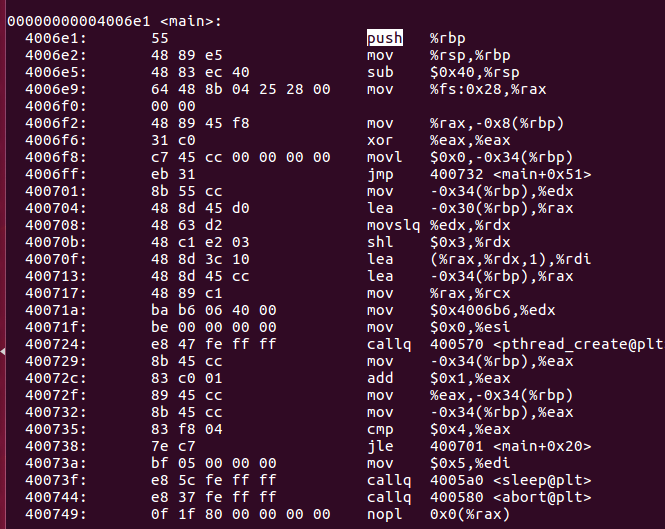
\includegraphics[scale=0.4]{slike/example_bp.png}
	\end{center}
	\caption{Primer1}
	\label{fig:primer1}
\end{figure}

Primera radi, želimo da postavimo tačku prekida na treću po redu instrukciju funkcije \emph{main}:

$48$ $          $ $89$ $          $ $e5$ $          $    $ mov$  $\%rsp,\%rbp$

Da bismo to uradili, menjamo prvi bajt instrukcije sa posebnom magičnom vrednošću, obično \emph{0xCC}, i kada izvršavanje dostigne do tog dela koda ono će se zaustaviti na tom mestu.

Pošto $0x48$ menjamo sa $0xcc$ i na tom mestu u kodu dobijamo instrukciju:

$cc$ $          $ $89$ $          $ $e5$ $          $    $ int3 $

Instrukcija $ int3 $ je posebna instrukcija Intel x86-64 procesorske arhitekture, koja izazva softverski prekid. Kada registar programski brojač (eng. \emph{CPU register pc}) stigne do $ int3 $ instrukcije izvršavanje se zaustavalja na toj tački. Dibager je već upoznat od strane korisnika i svestan je da je tačka prekida postavljena te isti čeka na signal koji ukazuje na to da je program dostigao do instrukcije prekida. Operativni sistem prepoznaje $ int3 $ instrukciju, poziva se specijalni obrađivač tog signala (na Linux sistemima \emph{do\_int3()}), koji dalje obaveštava debager šaljući mu signal sa kodom \emph{SIGTRAP} koji on obrađuje na željeni način. Treba napomenuti da ovo važi za Intel x86-64 procesorsku arhitekturu, instrukcija prekida za arhitekture kao što su ARM, MIPS, PPC itd., se drugačije kodira, ali postupak implementacije tačaka prekida je isti.

Ukoliko želimo da stavimo tačku prekida eksplicitno na funkciju \emph{main}, za to koristimo posrednika u vidu DWARF debug informacija. U tom slučaju debager traži element DWARF stabla koji ukazuje na informacije o \emph{main} funkciji, i odatle dohvata informaciju na kojoj adresi u memoriji se nalazi prva mašinska instrukcija date funkcije. Na slici \ref{fig:mainsub} vidimo DWARF element koji opisuje funkciju uz pomoć atributa. Dibager će pročitati \emph{DW\_AT\_low\_pc} atribut i na tu adresu postaviti $ int3 $ instrukciju. Napomenimo da DWARF debag simbole generišemo uz pomoć $ -g $ opcije kompajlera, ali o istim će biti opširnije u posebnoj sekciji.

\begin{figure}[h!]
	\begin{center}
		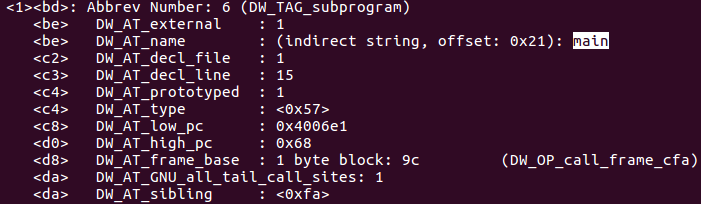
\includegraphics[scale=0.4]{slike/main_subprogram.png}
	\end{center}
	\caption{main DWARF subprogram}
	\label{fig:mainsub}
\end{figure}

Hardverske tačke prekida su direktno povezane sa hardverom u vidu specijalnih registara. Postavlja se na određenu adresu i harverski \emph{watchpoint} montri na zadatu adresu i može signalizirati razne promene na istoj, npr. čitanje, pisanje ili izvršavanje, što im daje prednost u odnosu na softverske tačke prekida. Mane u odnosu na softverske tačke prekida svakako jesu performanse, gde su neuporedivo sporije, i takođe neophodna hardverska podrška za korišćenje istih.

\subsection{Koračanje}

Pod procesom koračanja (eng. \emph{stepping}) kroz program podrazumevamo izvršavanje programa sekvencu po sekvencu. Sekvenca može biti jedna procesorska instrukcija, linija koda ili pak neka funkcija programa koji se debaguje.

Instrukcijsko koračanje na Intel x86-64 platformi je direktno omogućeno kroz sistemski poziv \emph{ptrace}:\newline\newline
\emph{ptrace(PTRACE\_SINGLESTEP, debuggee\_pid, nullptr, nullptr);}
\newline

Operativni sistem će dati signal kada je korak izvršen.

Pored instrukcijkog koračanja pomenućemo još jednu vrstu zakoračavanja u neku funkciju koja je pozvana $call$ ili $jump$ instrukcijom. Komanda koja nam to omogućava jeste \emph{step in}.

Treba napomenuti da postoje arhitekture za koje ovo ne važi, kao npr. ARM platforma, koja nema hardversku podršku za instrukcijsko koračanje i za njih se koračanje implementira na drugačiji način, uz pomoć emulacije instrukcija, ali u ovom radu neće biti opširnije o tome.

\subsection{Izlistavanje pozivanih funkcija}

Objasnimo komandu izlistavanje pozivanih funkcija (eng. \emph{backtrace}) posmatrajući organizaciju stek okvira (eng. \emph{stack frames}) na Intel x86-64 platformi.

\begin{figure}[h!]
	\begin{center}
		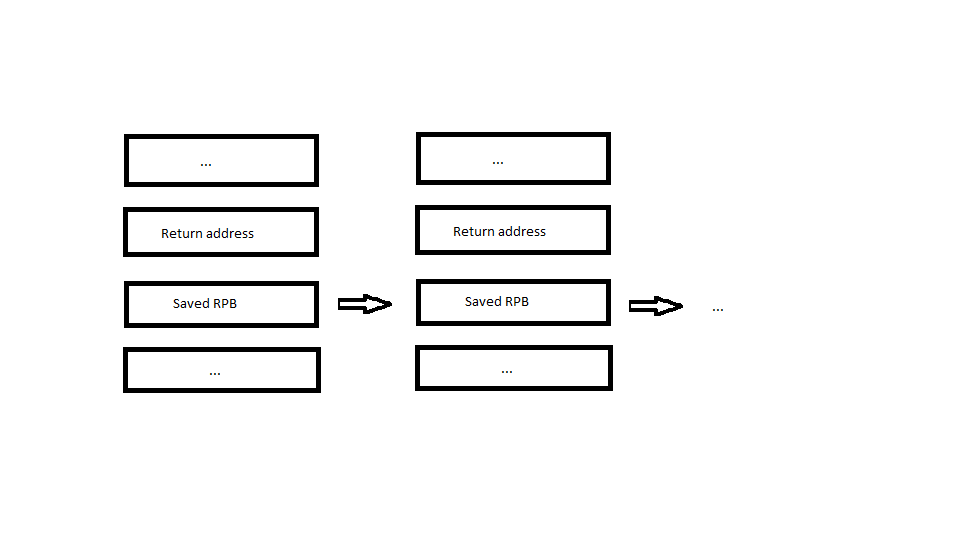
\includegraphics[scale=0.6]{slike/stack_frame.png}
	\end{center}
	\caption{Stek okviri}
	\label{fig:stack}
\end{figure}

Na slici \ref{fig:stack} navedeni su stek okviri za dva funkcijska poziva. Pre povratne vrednosti funkcije obično se ređaju argumenti funkcije. Sačuvana adresa u registru $RBP$ jeste adresa stek okvira svog pozivaoca. Prateći iste kao elemente povezane liste dolazimo do svih pozivanih funkcija do zadate tačke. Ako se pitamo kako debager ima informaciju o imenu funkcije odgovor je u tome što pretražuje DWARF stablo sa debag informacijama, tražeći \emph{DW\_TAG\_subprogram} sa odgovarajućom povratnom adresom, pritom čitajući \emph{DW\_AT\_name} atribut tog elementa.

\subsection{Čitanje vrednosti promenljivih}

Za čitanje vrednosti promenljivih u programu, debager pretražuje DWARF stablo tražeći promenljivu sa zadatim imenom. U slučaju lokalnih promenljivih, traži se \emph{DW\_TAG\_variable} element čiji \emph{DW\_AT\_name} odgovara navedenoj promenljivoj. Kada se ista pronađe konsultuje se \emph{DW\_AT\_location}, koji ukazuje na lokaciju gde se vrednost promenljive nalazi. Ukoliko ovaj atribut nije naveden debager će vrednost takve promenljive smatrati kao optimizovanu prijavljujući informaciju o tome.

\chapter{GNU GDB alat}
\label{chp:GDB}

\chapter{DWARF format}
\label{chp:DWARF}

\chapter{Datoteke jezgra}
\label{chp:corefiles}

\chapter{TLS}
\label{chp:TLS}

% ------------------------------------------------------------------------------

\section{Motivacija}
\section{Rukovanje TLS-om tokom izvršavanja programa}
\section{Arhitekturalno specifične zavisnosti}
\section{TLS Modeli pristupa}

\pangrami

\pangrami

\chapter{Implementacija rešenja}
\label{chp:Implementacija}

% ------------------------------------------------------------------------------
\chapter{Zaključak}
% ------------------------------------------------------------------------------
\pangrami

\pangrami

% ------------------------------------------------------------------------------
% Literatura
% ------------------------------------------------------------------------------
\literatura

% ==============================================================================
% Završni deo teze i prilozi
\backmatter
% ==============================================================================

% ------------------------------------------------------------------------------
% Biografija kandidata
\begin{biografija}
  \textbf{Vuk Stefanović Karadžić} (\emph{Tršić,
    26. oktobar/6. novembar 1787. — Beč, 7. februar 1864.}) bio je
  srpski filolog, reformator srpskog jezika, sakupljač narodnih
  umotvorina i pisac prvog rečnika srpskog jezika.  Vuk je
  najznačajnija ličnost srpske književnosti prve polovine XIX
  veka. Stekao je i nekoliko počasnih mastera.  Učestvovao je u
  Prvom srpskom ustanku kao pisar i činovnik u Negotinskoj krajini, a
  nakon sloma ustanka preselio se u Beč, 1813. godine. Tu je upoznao
  Jerneja Kopitara, cenzora slovenskih knjiga, na čiji je podsticaj
  krenuo u prikupljanje srpskih narodnih pesama, reformu ćirilice i
  borbu za uvođenje narodnog jezika u srpsku književnost. Vukovim
  reformama u srpski jezik je uveden fonetski pravopis, a srpski jezik
  je potisnuo slavenosrpski jezik koji je u to vreme bio jezik
  obrazovanih ljudi. Tako se kao najvažnije godine Vukove reforme
  ističu 1818., 1836., 1839., 1847. i 1852.
\end{biografija}
% ------------------------------------------------------------------------------

\end{document}